\documentclass[12pt, a4paper]{article}
\usepackage[print,sort]{standalone}
\usepackage[T1]{fontenc}
\usepackage[utf8]{inputenc}
\usepackage[english]{babel}
\usepackage{graphicx,float}
\usepackage{amssymb}
\usepackage{amsmath,cancel}
\usepackage{mathrsfs}
\usepackage{epstopdf}
\usepackage{subcaption}
\usepackage{slashed}
\usepackage{hhline}
\usepackage[margin=1.2in]{geometry}
\usepackage[hidelinks]{hyperref}
\usepackage{wrapfig}


\hfuzz=5pt


\begin{document}

\begin{titlepage}
\begin{center}
\vspace*{3cm}
\Huge
\textbf{Project 4} \\
\Large  
FYS4150 Computational Physics 
\vspace*{3cm} \\ 

Even S. Håland 
\vspace*{5cm} \\

\normalsize
\section*{Abstract}

In this project we perform Monte Carlo simulations of magnetic systems using the Ising model. We do 
comparisons between our simulations and an analytically solvable system, as well as studies of 
equilibration time for larger systems. We also study phase transitions in the model, and estimate 
the critical temperature in the thermodynamical limit to be $k_BT_C/J=2.269$, which is in very good 
agreement with the exact value for this quantity. 

\end{center}
\end{titlepage}

\section{Introduction}

The aim of this project is to do Monte Carlo simulations of magnetic systems described by the 
two-dimensional Ising model. The Ising model describes binary systems, that is a collection of objects 
with only two possible states each. Here we will take these two states to be spin-up and spin-down. In
particular we will study phase transitions in such systems. 

We will start by studying some analytical solutions to the Ising model by considering a $2\times 2$ 
lattice. Then we will make a code that simulates the evolution of such systems for larger lattices. We 
will see how the system evolves depending on temperature and the initial state of the system, and we 
will finally study phase transitions, and extract the critical temperature for phase transitions in 
the thermodynamical limit.  

In our simulations we will use the Metropolis algorithm for accepting or rejecting the Monte Carlo 
trials. We will also, as these simulations are quite time consuming, parallelize the code, so that 
we can distribute our jobs to multiple processors. 

\section{Theoretical framework}

\subsection{The Ising model}

As mentioned in the introduction the Ising model describes a collection of objects, where each object 
can take two values, i.e. spin-up and spin-down, parametrized by $s=\pm 1$. We will consider a 
two-dimensional model with the spins organized in a square lattice with dimension $L$, so the total 
number of spins is given by $N = L\times L$. The two key quantities for describing our system 
will be energy and magnetization. The total energy of this system (with no external magnetic field) 
is given by 
\begin{align}
E = -J\sum_{<kl>}^{N} s_k s_l, 
\end{align}
where $J$ is a coupling constant and $<kl>$ indicates that we sum over neighbouring spins only, i.e. 
an object is only "talking" to its closest neighbours. The total magnetization of the system is simply 
given by the sum over all spins: 
\begin{align} 
M = \sum_k^N s_k. 
\end{align}

A natural next step is to calculate expectation values within this theory, i.e. mean energy, 
$\left\langle E \right\rangle$, and mean magnetization $\left\langle M \right\rangle$. To be able to do 
so we need to introduce some concepts from statistical physics.  

\subsection{Elements from statistical physics}

In order to calculate expectation values we need a probability distribution. In our case this is the 
Boltzmann distribution, given as 
\begin{align*}
P_i(\beta) = \frac{e^{-\beta E_i}}{Z}, 
\end{align*}
where $\beta = 1/k_B T$ (where $k_B$ is Boltzmann's constant and $T$ is temperature), $E_i$ is the 
energy of state $i$ and $Z$ is the partition function. The partition function is given as 
\begin{align*}
Z = \sum_{i=1}^n e^{-\beta E_i}, 
\end{align*}
where the sum runs over all possible (micro)states of the system. The expectation value of some 
general quantity $A$ can now be calculated as 
\begin{align*}
\left\langle A \right\rangle = \sum_{i=1}^n A_i P_i(\beta) = \frac{1}{Z} \sum_{i=1}^n A_i e^{-\beta E_i}, 
\end{align*} 
and the variance of $A$ is given as 
\begin{align*}
\sigma_A^2 = \left\langle A^2 \right\rangle - \left\langle A \right\rangle^2. 
\end{align*}
By considering the variances of $E$ and $M$ we can also calculate specific heat, $C_V$, and 
susceptibility, $\chi$, as 
\begin{align*}
C_V = \frac{1}{k_BT^2}\sigma_E^2 \quad \text{and} \quad \chi = \frac{1}{k_B T}\sigma_M^2. 
\end{align*}

\subsection{Analytical solutions}

Using the above described framework we can study the Ising model for a $2\times 2$ lattice analytically. 
This means that we have $4$ objects which each can have $s=\pm 1$. Both in this and later analysis we 
will make use of so-called periodic boundary conditions, which means that we let the first and last 
spins in a lattice row be neighbours when summing up the energy. 

We label the spins in the $2\times 2$ lattice with $k \in \left\lbrace 1,2,3,4\right\rbrace$, and the 
energy is then given by 
\begin{align*}
E & = -J(s_1 s_2 + s_2 s_1 + s_1 s_3 + s_3 s_1 +s_2 s_4 +s_4 s_2 + s_3 s_4 + s_4 s_3) \\
  & = -2J(s_1 s_2 + s_1 s_3 + s_2 s_4 + s_3 s_4),  	
\end{align*}  
and the magnetization as 
\begin{align*}
M = s_1 + s_2 + s_3 + s_4. 
\end{align*}

\begin{table}[H]
\caption{Degeneracy, energy and magnetization for the different spin configurations in the $2\times 2$
lattice.}
\label{tab:2times2}
\begin{center}
\begin{tabular}{cccc} \hline\hline
$\#$ spin-up & Degeneracy & $E$ & $M$ \\ \hline
$4$ & $1$ & $-8J$ & $4$ \\ 
$3$ & $4$ & $0$ & $2$ \\
$2$ & $2$ & $8J$ & $0$ \\  
$2$ & $4$ & $0$ & $0$ \\ 
$1$ & $4$ & $0$ & $-2$ \\ 
$0$ & $1$ & $-8J$ & $-4$ \\ \hline
\end{tabular}
\end{center}
\end{table}

Table \ref{tab:2times2} lists the possible values for these quantities for all possible spin 
configurations, along with the degeneracy for each spin configuration. Using this we find that the 
partition function is given as 
\begin{align*}
Z = 12 + 2e^{8J\beta} + 2e^{-8J\beta} = 12 + 4 \cosh(8J\beta). 
\end{align*} 
Using this along with the expressions from the previous section we can calculate 
$\left\langle E \right\rangle$, $\left\langle |M| \right\rangle$, $C_V$ and $\chi$, and we arrive 
to the following expressions:  
\begin{align*}
\left\langle E \right\rangle = -\frac{8J\cosh (8\beta J)}{3 + \cosh (8\beta J)}  
\end{align*}  
\begin{align*}
\left\langle |M| \right\rangle = \frac{4+2 e^{8\beta J}}{3 + \cosh (8\beta J)}  
\end{align*} 
\begin{align*}
C_V = \frac{192J^2\sinh (8\beta J)}{k_BT^2\left[ 3 + \cosh (8\beta J)\right]^2}  
\end{align*} 
\begin{align*}
\chi = \frac{4\beta\left( 1 + 2e^{8J\beta} \right)}{3 + \cosh (8\beta J)}
\end{align*}
These expressions (with inserted values for $T$ and $J$) can be used as a check on our simulations.   

\subsection{Phase transitions}

In important part of this project is to study phase transitions in our system. The Ising model with 
no external magnetic field undergoes a second order phase transition at some critical temperature, $T_C$, 
which is such that $\left\langle M \right\rangle=0$ for $T>T_C$. In the thermodynamical limit 
(i.e. $L\rightarrow\infty$) $C_V$ and $\chi$ are divergent at $T_C$. The lattices we study here will 
(of course) be of finite dimensions, and  $C_V$ and $\chi$ will not diverge, but rather show a 
maximum around $T_C$. 

The critical temperature is given by  
\begin{align}
T_C(L) - T_C(L=\infty) = aL^{-1/\nu}
\label{eq:T_C}
\end{align}
where $a$ is a constant and $\nu$ is given by 
\begin{align*}
\xi(T) = |T_C - T|^{-\nu}, 
\end{align*}
where $\xi$ is called the \textit{correlation length}, which defines the length scale at which microscopic 
variables are correlated. By measuring the critical temperature for finite sized lattices we can 
extract $T_C$ in the thermodynamical limit ($T_C(L=\infty)$), which is done towards the end of the 
result section. We do 
however need estimates of $T_C$ for two different $L$'s, since equation \ref{eq:T_C} contains two 
unknown quantities ($T_C(L=\infty)$ and $a$). The exact result (calculated by Lars Onsager) is given by 
\begin{align}
k T_C/J = \frac{2}{\ln(1+ \sqrt{2})} \approx 2.269
\end{align}
when $\nu = 1$. 

\section{Code}

All code written for the project can be found in the following git-repository:  \vspace{0.5cm} \\ 
\fbox{
\href{https://github.com/evensha/FYS4150/tree/master/Project4/Programs}
{https://github.com/evensha/FYS4150/tree/master/Project4/Programs} 
} \vspace{0.5cm} \\ 
The three most important scripts in this repository are: 
\begin{itemize}
\item \texttt{main.cpp}
\item \texttt{Plotting.py}
\item \texttt{Phase\_trans.py}
\end{itemize}
The first one is the C++ program that performs the Monte Carlo simulation, while the two other are 
python scripts used for evaluating and plotting the output from the simulation. 

The repository also contains the C++ library (\texttt{lib.cpp}/\texttt{lib.h}) provided for the course, 
as well as a \texttt{makefile} and the executable file \texttt{Program.x}. 

\subsection{The main program}

The set-up of the simulation (i.e. the \texttt{main.cpp} program) follows very closely the approach from 
the example programs in Chapter $13$ of the lecture notes \cite{Lecture Notes}, but with some 
modifications. Paralleliziation of the program using Open MPI is also implemented as suggested in 
the lecture notes. A slight difference is however the usage of Armadillo \cite{Armadillo} for handling 
vectors and matrices.   

The first thing we do in the main program is to define some useful functions:  
\begin{itemize}
\item \texttt{periodic}: Handles the periodic boundary conditions when summing up the energy of a lattice.
\item \texttt{initialize}: Initialize the spin matrix and calculates initial energy and magnetization. 
The spin matrix is initialized either with ordered spins (all spins up), or a random spin configuration. 
Random spins are generated using the \texttt{ran1} function from the library (\texttt{lib.cpp}).
\item \texttt{Metropolis}: Implements the Metropolis algorithm with the Metropolis test. This will be 
discussed in a bit more detail later. 
\item \texttt{output}: Write final output (e.g. mean $E$ and $M$, $C_V$ and $\chi$) to file. 
\end{itemize}
The three latter functions are implemented in the end of the program. 

Next we enter the main function. This function takes three input arguments: lattice size, number of 
Monte Carlo cycles and an integer which indicates whether or not we want a random initial spin state. 
In the beginning of this function we set up all necessary quantities, vectors and matrices, and we 
also initialize MPI. 

Then we start a loop over the temperatures we want to consider. In our analysis we will mostly 
consider two situations; either a lattice with $L=20$ and temperatures $T=1.0$ and $T=2.4$, or 
larger lattices with $L=40,60,80,100$ and $T \in \left[2.0,2.3\right]$. For this reason the program 
is tailored so that the temperatures taken into account depends on the lattice size given as input. 

For each new temperature we call the \texttt{initialize} function, and we also set up an array 
containing the five possible energy differences (or rather the 
ratios between probabilities for different energies, $\exp(-\beta\Delta E)$), and an array for 
storing the final average values for a given temperature. Then we call the initialize function which 
calculates initial energy and magnetization. 
For the $L = 20$ case we would like to study the evolution of the mean values, so in this case we make 
an output file to which we write updated average values after each MC cycle.

Finally we are ready to start running the simulation. For each cycle we call the  
\texttt{Metropolis} function, update the average values and write to file (if required). When the 
MC loop is finished we write the final average values to file, and move to the next temperature.  
  
\subsection{The Metropolis algorithm}

As mentioned the Metropolis algorithm \cite{Metropolis} is implemented in the \texttt{Metropolis} 
function. The idea of this algorithm is briefly explained in the following. 

We start by establishing an initial state with some energy, $E_0$, which is done in the 
\texttt{initialize} function. Then we loop over the total number of spins. For each turn in the loop 
we pick out a random lattice position, and try to flip this spin. Then we compute the new energy, $E_1$, 
and look at the energy difference between the new and the previous state, $\Delta E = E_1 - E_0$. 
If $\Delta E\leq 0$ we accept the new spin configuration, while if $\Delta E > 0$ we pick a random 
number $r$, and compare it to the probability ratio $w=\exp(-\beta\Delta E)$. If $r\leq w$ we 
accept the configuration. 

Whenever a configuration is accepted we need to update energies and magnetization. The algorithm is 
then repeated until we get the desired precision in our simulation. Each loop over total number of spins 
is called a \textit{Monte Carlo cycle}.     

\section{Results}

We previously calculated analytical expressions for the expectation values of $E$ and $|M|$, as well as 
the heat capacity, $C_V$, and the susceptibility, $\chi$. By inserting $T = 1.0$ and $J=k_B = 1.0$ 
in these expressions we can compare the values with those obtained in our MC simulation. ($J=k_B = 1.0$ 
are used in all calculations and simulations in this project.) This is done in 
Table \ref{tab:analytical_vs_sim} for various number of MC cycles. We see that by using a million 
MC cycles we get good agreement between analytical and simulated values. 

\begin{table}[ht!]
\caption{Comparison between analytically calculated and simulated expectation values for the various 
thermodynamical quantities for the $2\times 2$ lattice.}
\label{tab:analytical_vs_sim}
\begin{center}
\begin{tabular}{ccccc} \hline\hline
 & & \multicolumn{3}{c}{$\#$ MC cycles} \\ 
Parameter & Analytical value & $10^4$ & $10^5$  & $10^6$ \\ \hline
$\left\langle E \right\rangle$ & $-7.984$ & $-7.967$ & $-7.982$ & $-7.984$ \\ 
$\left\langle |M| \right\rangle$ & $3.995$  & $3.989$  & $3.994$  & $3.995$  \\
$C_V$                          & $0.128$  & $0.261$  & $0.141$  & $0.129$  \\
$\chi$						   & $15.97$  & $15.93$  & $15.95$  & $15.97$  \\ \hline\hline
\end{tabular}
\end{center}
\end{table}

Now that we have established that our algorithm is able to produce reasonable results we would like 
to extend the lattice. We start by considering $L=20$, and want to see how many MC cycles we need for the 
system reach equilibrium by studying the evolution of the mean energy and the mean magnetization.  
Results for two different temperatures ($T=1.0$ and $T=2.4$) are shown in Figure \ref{fig:L20_ordered} 
(all spins up initially) and Figure \ref{fig:L20_random} (random initial spins). 

\begin{figure}[ht!]
	\centering
  	\begin{subfigure}[b]{0.495\textwidth}
		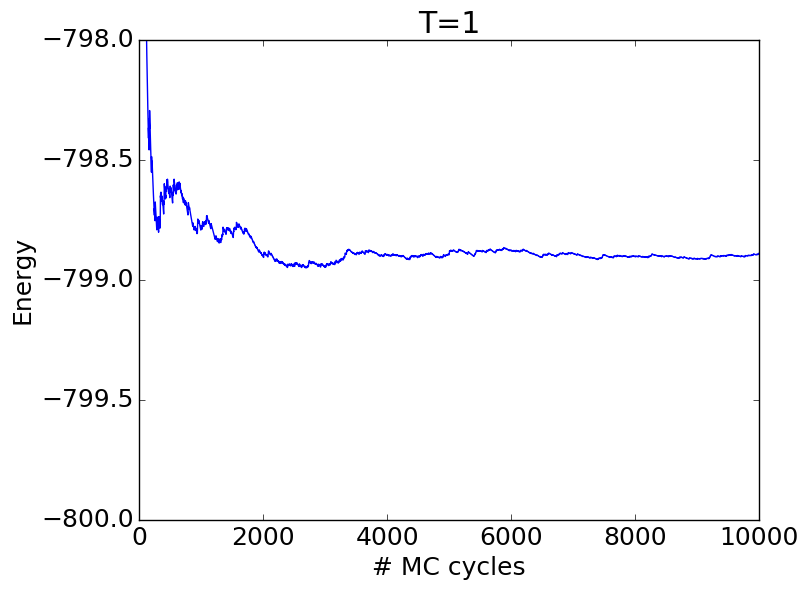
\includegraphics[width=\textwidth]{../Programs/Output/Energy_ordered_1.png}
        %\caption{}
        %\label{}
  	\end{subfigure}
  	\begin{subfigure}[b]{0.495\textwidth}
		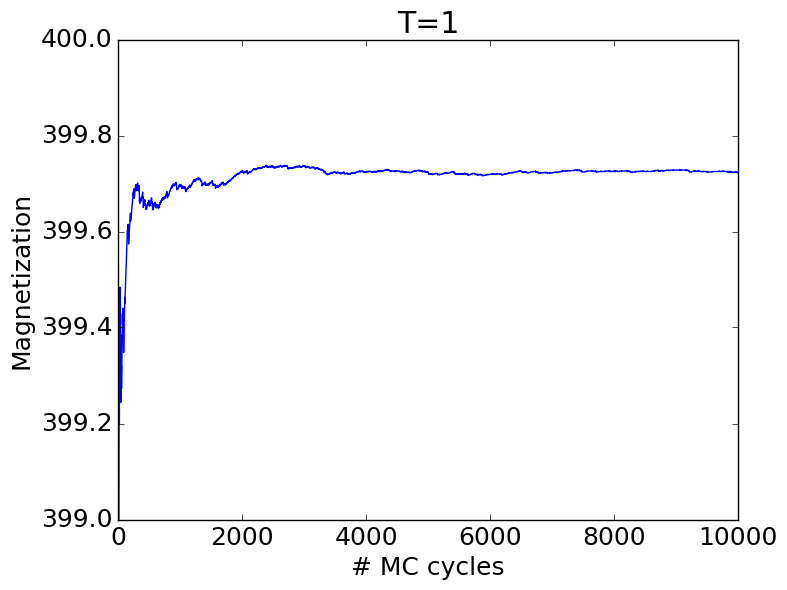
\includegraphics[width=\textwidth]{../Programs/Output/Magnetization_ordered_1.png}
        %\caption{}
        %\label{}
  	\end{subfigure}
  	\begin{subfigure}[b]{0.495\textwidth}
		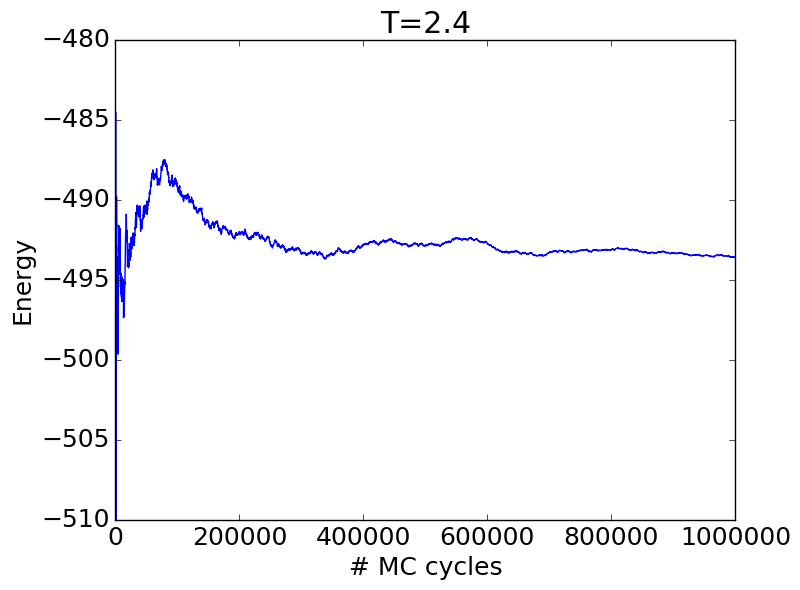
\includegraphics[width=\textwidth]{{../Programs/Output/Energy_ordered_2.4}.png}
        %\caption{}
        %\label{}
  	\end{subfigure}
  	\begin{subfigure}[b]{0.495\textwidth}
		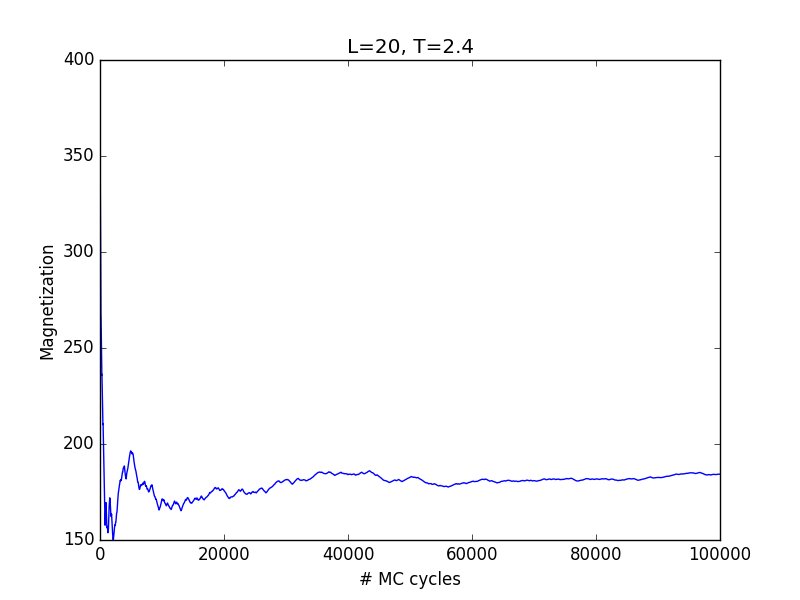
\includegraphics[width=\textwidth]{{../Programs/Output/Magnetization_ordered_2.4}.png}
        %\caption{}
        %\label{}
	\end{subfigure}
	\caption{Mean energy and magnetization as function of number of MC cycles for $L=20$ for 
	two different temperatures with all spins up initially.}
	\label{fig:L20_ordered}
\end{figure}

\begin{figure}[ht!]
	\centering
  	\begin{subfigure}[b]{0.495\textwidth}
		
\includegraphics[width=\textwidth]{../Programs/Output/Energy_random_1.png}
        %\caption{}
        %\label{}
  	\end{subfigure}
  	\begin{subfigure}[b]{0.495\textwidth}
		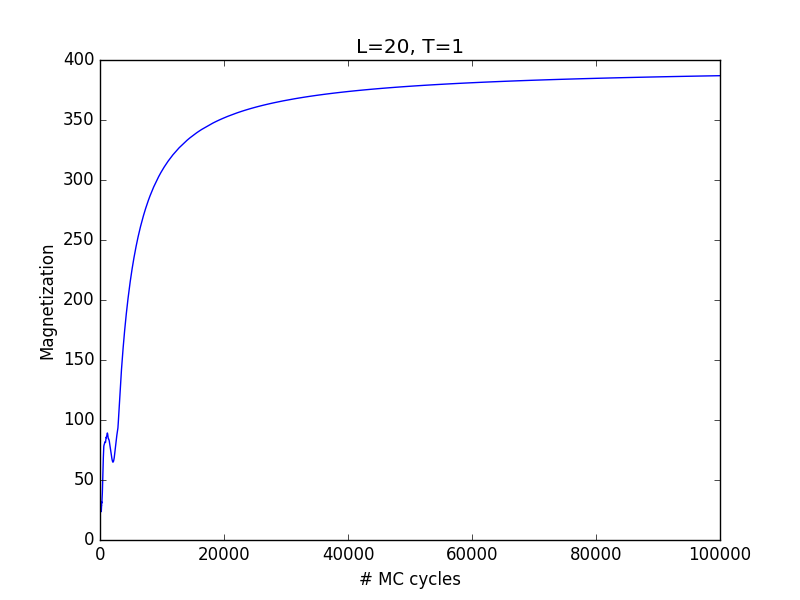
\includegraphics[width=\textwidth]{../Programs/Output/Magnetization_random_1.png}
        %\caption{}
        %\label{}
  	\end{subfigure}
  	\begin{subfigure}[b]{0.495\textwidth}
		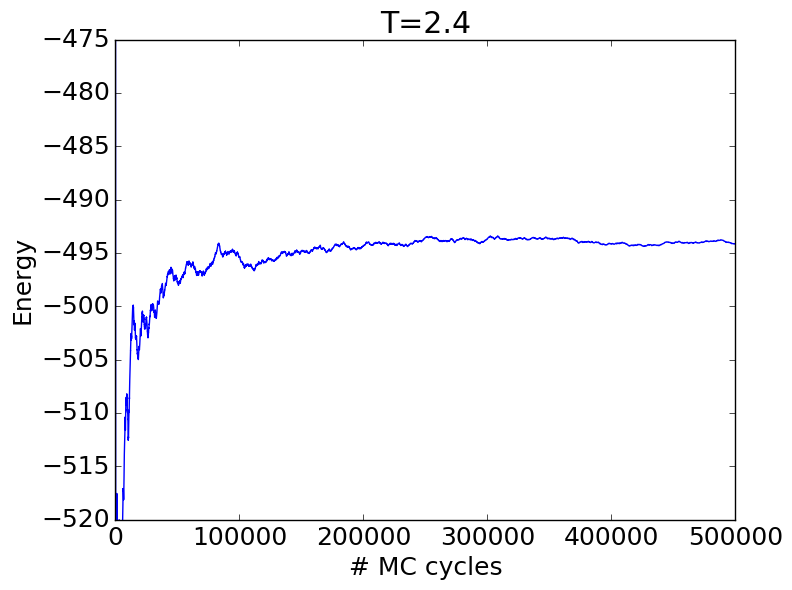
\includegraphics[width=\textwidth]{{../Programs/Output/Energy_random_2.4}.png}
        %\caption{}
        %\label{}
  	\end{subfigure}
  	\begin{subfigure}[b]{0.495\textwidth}
		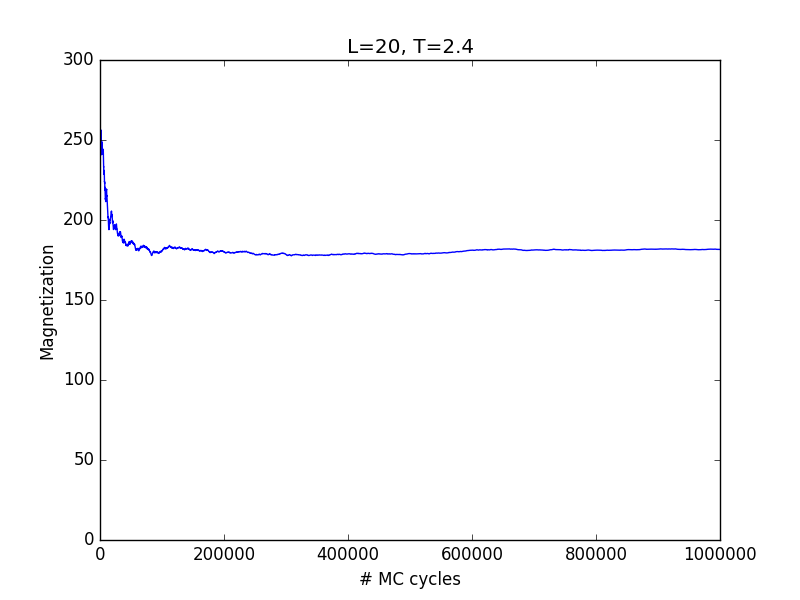
\includegraphics[width=\textwidth]{{../Programs/Output/Magnetization_random_2.4}.png}
        %\caption{}
        %\label{}
	\end{subfigure}
	\caption{Mean energy and magnetization as function of number of MC cycles for $L=20$ for 
	two different temperatures with random initial spins.}
	\label{fig:L20_random}
\end{figure}

When starting with all spins up we see that the averages stabilizes quite fast when $T=1.0$ 
($\sim 3,000$ MC cycles), while it takes considerably longer when $T=2.4$ ($\sim 300,000$ MC cycles).
We also see that for $T=2.4$ there are more fluctuations, also after the stable state is reached
With random initial spins we see that we get very smooth curves for $T=1.0$. This is probably because 
the most likely states are reached quite quickly, so the energy/magnetization stays more or less the 
same, so that the average is smoothly converging. However, for $T=2.4$ we again see more fluctuations, 
but the equilibrium is actually reached faster than with ordered initial spins. 

The behaviour we observe is governed by the Boltzmann distribution, $e^{-E/k_BT}$. This basically tells 
us that by increasing the temperature we increase the likelihood for entering a larger number of 
states. This is also supported by Figure \ref{fig:Acc_confs}, which shows how the number of accepted 
states in our simulation evolves with number of MC cycles, as well as Figure \ref{fig:E_prob_dist}, 
which shows the energy probability distribution. The variances for the energies is calculated to 
be $\sigma_E^2(T=1.0)=8.6$ and $\sigma_E^2(T=2.4)=3219$, which is also in good correspondence with 
Figure \ref{fig:E_prob_dist}, as energies varies much more when the temperature is increased.     

\begin{figure}
\begin{center}
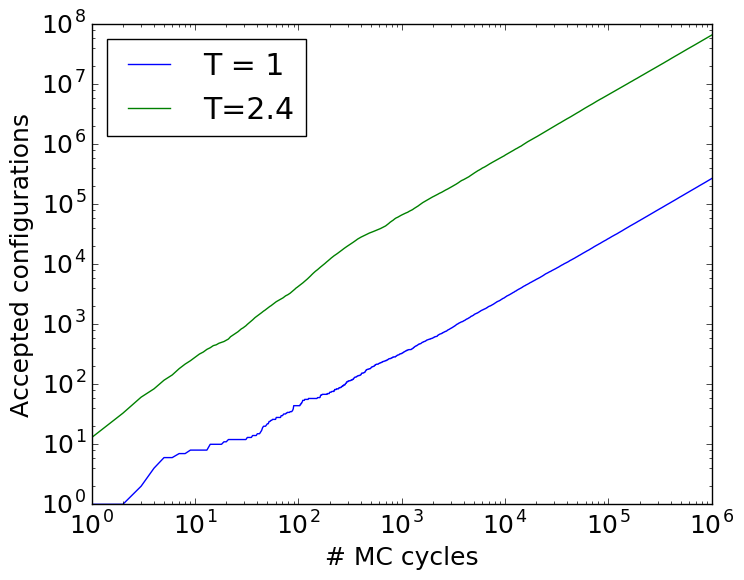
\includegraphics[scale=0.5]{../Programs/Output/Accepted_configurations.png}
\caption{Number of accepted spin configurations for $T=1.0$ and $T=2.4$.}
\label{fig:Acc_confs}
\end{center}
\end{figure}

\begin{figure}
	\centering
  	\begin{subfigure}[b]{0.495\textwidth}
		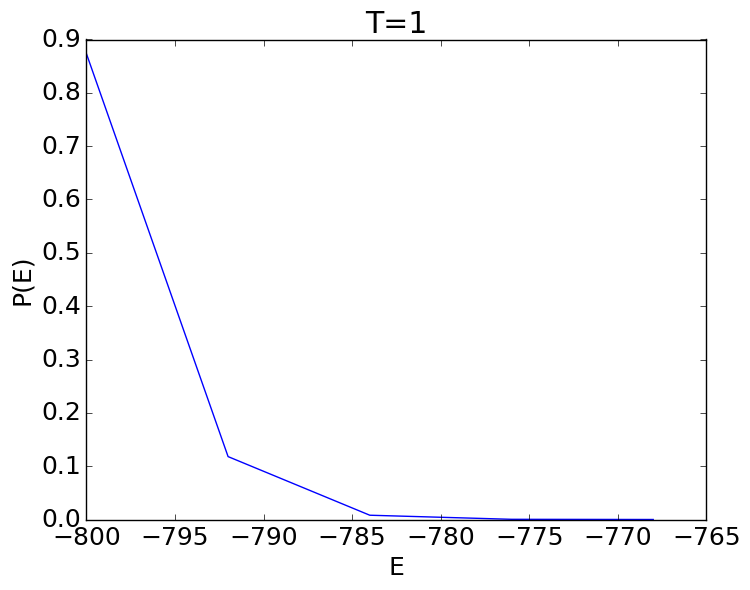
\includegraphics[width=\textwidth]{../Programs/Output/Energy_PDF_T=1.png}
        %\caption{}
        %\label{}
  	\end{subfigure}
  	\begin{subfigure}[b]{0.495\textwidth}
		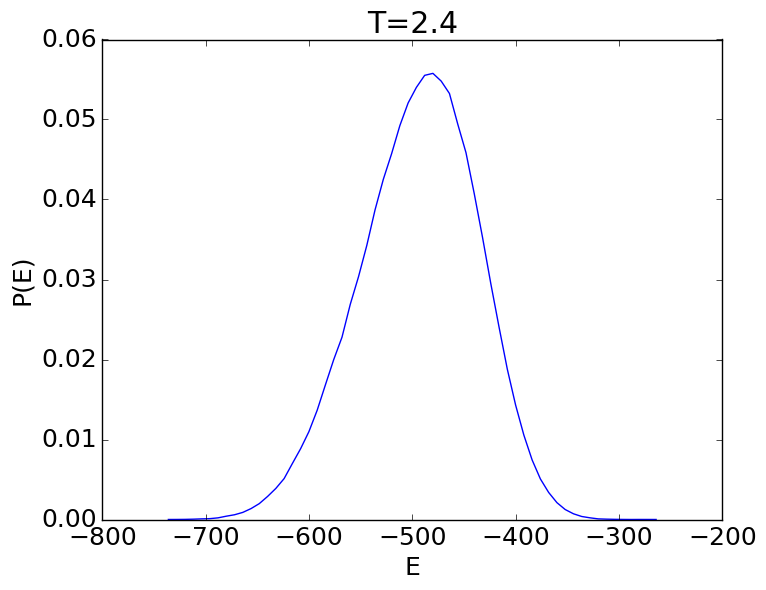
\includegraphics[width=\textwidth]{{../Programs/Output/Energy_PDF_T=2.4}.png}
        %\caption{}
        %\label{}
  	\end{subfigure}
  	\caption{Probability distribution for energy states with $T=1.0$ and $T=2.4$.}	
  	\label{fig:E_prob_dist}
\end{figure}

\subsection{Phase transitions}

Finally we will have a look at phase transitions in the Ising model. In Figure \ref{fig:phase} 
the quantities $\left\langle E \right\rangle$, $\left\langle |M| \right\rangle$, $C_V$ and $\chi$ are 
plotted as function of temperature for four different lattices sizes, $L=40,60,80,100$. The 
simulations are done with a temperature step of $\Delta T = 0.01$, and with $5\cdot 10^5$ MC cycles for 
$L=40,60,80$ and $10^6$ MC cycles for $L=100$. Both $C_V$ and $\chi$ peaks towards the end of the 
temperature range, while the magnetization falls towards zero, indicating a phase transition. 

\begin{figure}
	\centering
  	\begin{subfigure}[b]{0.495\textwidth}
		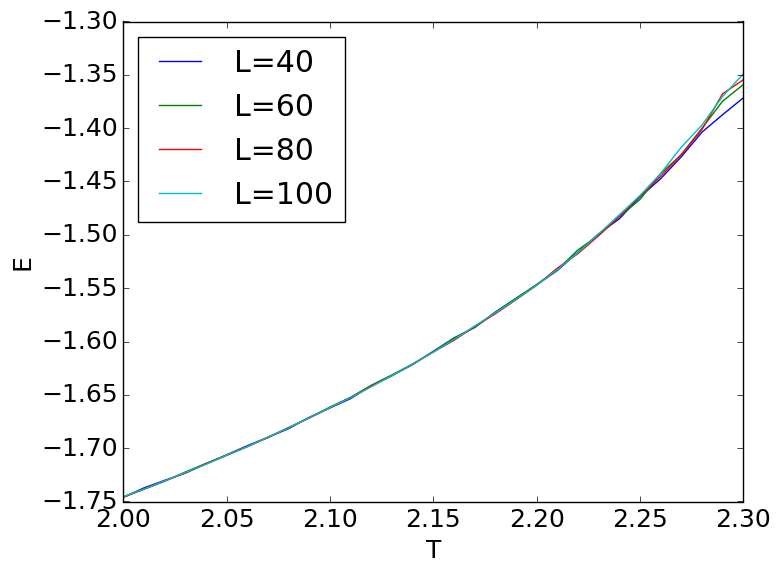
\includegraphics[width=\textwidth]{{../Programs/Output/E_T}.png}
        %\caption{}
        %\label{}
  	\end{subfigure}
  	  	\begin{subfigure}[b]{0.495\textwidth}
		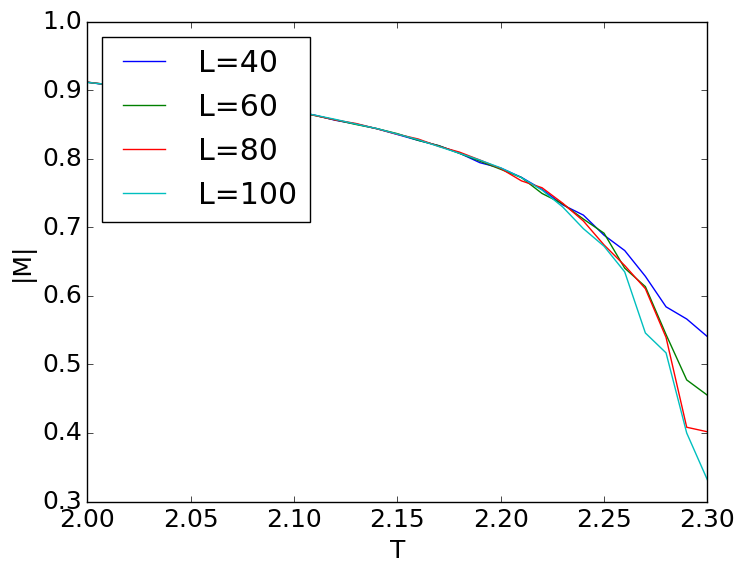
\includegraphics[width=\textwidth]{{../Programs/Output/M_T}.png}
        %\caption{}
        %\label{}
  	\end{subfigure}
  	\begin{subfigure}[b]{0.495\textwidth}
		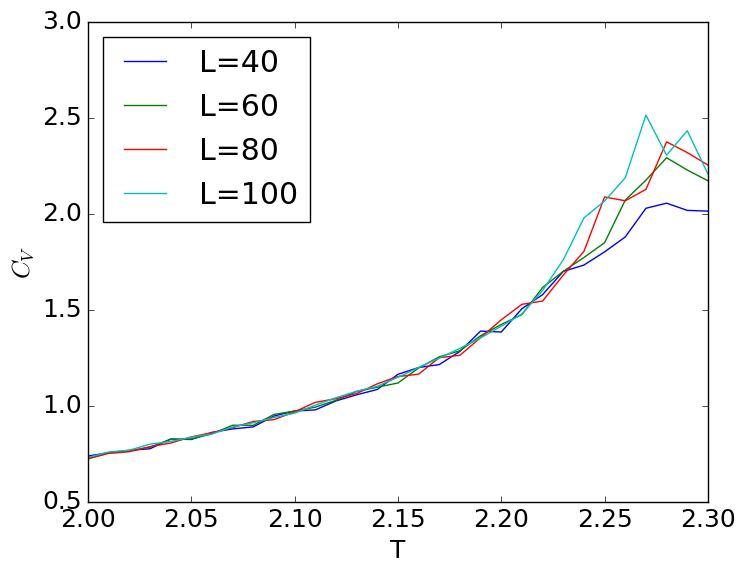
\includegraphics[width=\textwidth]{{../Programs/Output/CV_T}.png}
        %\caption{}
        %\label{}
  	\end{subfigure}
  	\begin{subfigure}[b]{0.495\textwidth}
		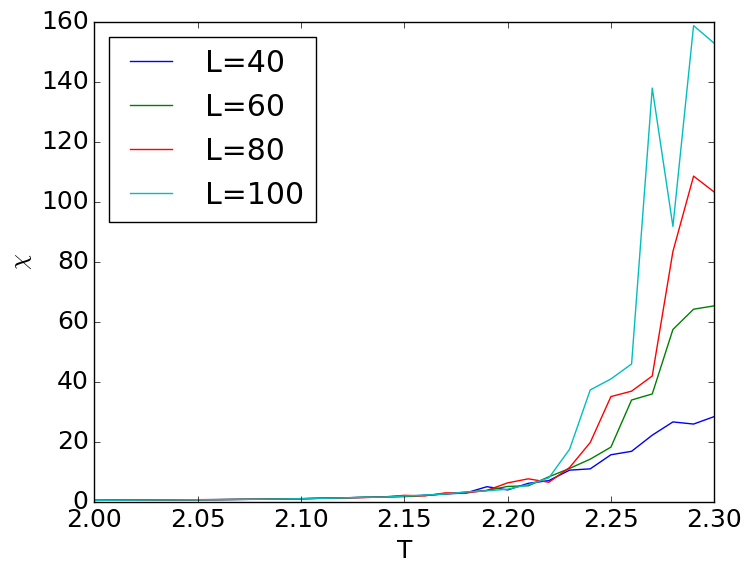
\includegraphics[width=\textwidth]{{../Programs/Output/Chi_T}.png}
        %\caption{}
        %\label{}
  	\end{subfigure}  	
  	\caption{$\left\langle E \right\rangle$, $\left\langle |M| \right\rangle$, $C_V$ and $\chi$
  	plotted as function of temperature for various lattice sizes.}
  	\label{fig:phase}  		
\end{figure}

However, the curves are not exactly beautiful, which could probably be improved by increasing the number 
of MC cycles. This was not done due to the time consumption of these simulations, in particular for the 
largest lattices, even though our program is parallelized. Time consumption for simulation of a 
$L=40$ lattice with $500,000$ MC cycles is shown in Table \ref{tab:time}, using $1$, $2$ and $4$ 
processors. When moving from one to two processors we see that we get a very nice speed up, i.e. the 
time is decreased by a factor of $\sim 2$. When moving to four processors we are able to speed it up 
a little bit more. However, four is the total number of processors on my laptop, meaning that the full 
capacity of all four processors will not be used for the MC simulation.          
\begin{table}
\caption{Time consumption for simulation of $500,00$ MC cycles of a $L=40$ lattice, using different 
number of processors.}
\label{tab:time}
\begin{center}
\begin{tabular}{cc} \hline\hline
$\#$ processors & Time \\ \hline 
$1$ & $24.6$ min \\
$2$ & $12.4$ min\\
$4$ & $9.8$ min\\ \hline 
\end{tabular}
\end{center}
\end{table}

The final step is to extract the critical temperature in the thermodynamical limit, as discussed in 
section 2.4. When doing these calculations we need somewhat higher precision in the estimates of 
$T_C$, so it is practical (since we have established the approximate values of $T_C$ from Figure
\ref{fig:phase}) to run the simulations again with the same number of MC cycles, but with 
$T\in [2.65,2.85]$ and $\Delta T = 0.001$. By looking at $C_V$ in the output files for $L=60$ and $L=100$
(found as \texttt{Output\_L\_60\_dt0.001.txt} and \texttt{Output\_L\_60\_dt0.001.txt} in the 
Output folder in the previously mentioned git repository) we find that $T_C(L=60)=2.279$ and 
$T_C(L=100)=2.275$. Using these values together with Equation \ref{eq:T_C} gives us 
\begin{align*}
T_C(L=\infty) = \frac{2.279 - 100/60\cdot 2.275}{1- 100/60} = 2.269, 
\end{align*}
as critical temperature in the thermodynamical limit, 
which is precisely the same as the exact result. (I'm a bit surprised that the estimation was \textit{that}
accurate. It is not clear to me if this is some sort of magic coincidence from my numbers, or if 
the simulation actually is that good.) 

\section{Summary and conclusions}

In this project we have done Monte Carlo simulations of magnetic systems by using the Ising model. We 
found that we are able to obtain good precision in our simulations, compared to analytical values 
for a $2\times 2$ lattice. We have also seen that the time needed to reach equilibrium depends on both 
initial spin configuration and temperature, and that by increasing the temperature the energy will 
fluctuate more, as more states are available, as described by the Boltzmann distribution. 

A key point of the project was the studies phase transitions in our systems, and we have extracted 
the critical temperature for such in the thermodynamical limit with surprisingly good precision. 
Finally, we have also seen that Monte Carlo simulation can be quite time consuming, meaning that
parallelization of the program is of great value. 

\begin{thebibliography}{40}

\bibitem{Lecture Notes} M. Hjort-Jensen (2015), \textit{Computational Physics - Lecture Notes Fall 2015}, 
Department of Physics, University of Oslo. \\ 
\href{https://github.com/CompPhysics/ComputationalPhysics/blob/master/doc/Lectures/lectures2015.pdf}
{https://github.com/CompPhysics/ComputationalPhysics/blob/master\\/doc/Lectures/lectures2015.pdf}

\bibitem{Armadillo} C. Sanderson, R. Curtin (2016), Armadillo: a template-based C++ library for linear 
algebra, \textit{Journal of Open Source Software}, Vol. 1, p. 26.  

\bibitem{Metropolis} N. Metropolis et al. (1953), Equation of State Calculations by Fast Computing 
Machines, \textit{The Journal of Chemical Physics}, Vol. 21(6), p. 1087. \\
\href{https://doi.org/10.1063/1.1699114}{https://doi.org/10.1063/1.1699114}
 

\end{thebibliography} 

\end{document}
